\documentclass[a4paper,11pt]{article}
\usepackage[T1]{fontenc}
\usepackage[utf8]{inputenc}
\usepackage{lmodern}

\usepackage{amsmath}
\usepackage{amsthm}

\usepackage{graphicx}
\graphicspath{{../data/}}
\usepackage{caption}
\usepackage{subcaption}

\usepackage{fullpage}

\renewcommand{\thesubsection}{\alph{subsection}}

\title{Image Processing 1 - Exercise 4 - WiSe 2012/13}
\author{Weipeng He \\ \texttt{2he@informatik.uni-hamburg.de} \\ \texttt{6411529}}

\begin{document}

\maketitle

\section{}
\subsection{}
The grayvalues will be extended for 0 to 255. As the original values are equally spaced, so are the egalized values, which are 0, 85, 170, 255.

\subsection{}
The optical effect is that the contrast becomes higher.

\subsection{}
The image after histogram egalization will stay the same as the grayvalues are also equally spaced.

\subsection{}
Please refer to source code in \texttt{src/egalize.py} and result images in \texttt{data/}.

\begin{figure}[h]
\centering
\begin{subfigure}[b]{.45\textwidth}
  \centering
  
\includegraphics[width=.8\textwidth]{pic1}
  \caption{Original Picture 1 (50, 100, 150, 200)}
\end{subfigure}
\begin{subfigure}[b]{.45\textwidth}
  \centering
  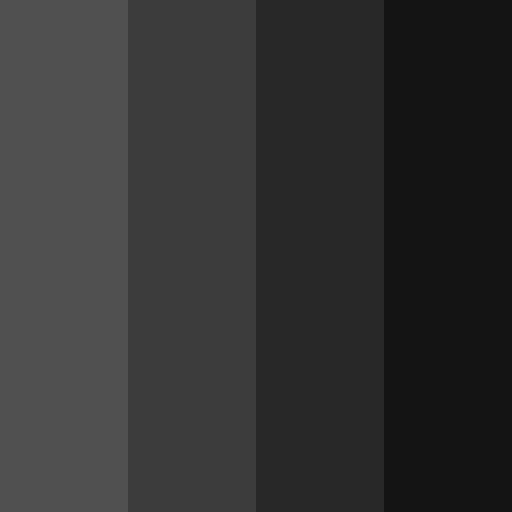
\includegraphics[width=.8\textwidth]{pic2}
  \caption{Original Picture 2 (20, 40, 60, 80)}
\end{subfigure}

\begin{subfigure}[b]{.45\textwidth}
  \centering
  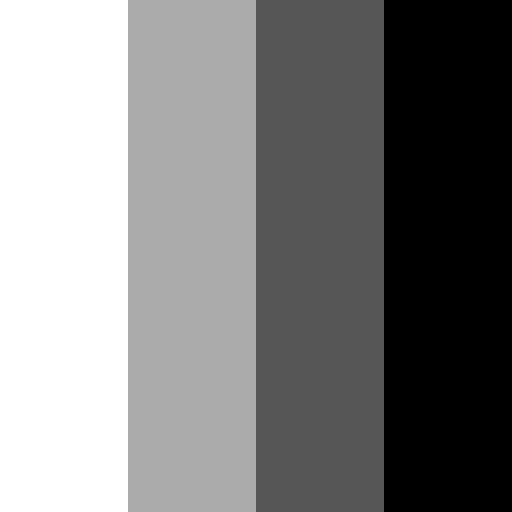
\includegraphics[width=.8\textwidth]{pic1_egal}
  \caption{Egalized Picture 1}
\end{subfigure}
\begin{subfigure}[b]{.45\textwidth}
  \centering
  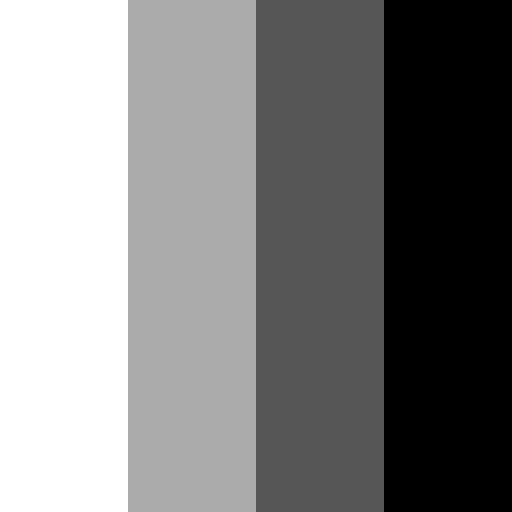
\includegraphics[width=.8\textwidth]{pic2_egal}
  \caption{Egalized Picture 2}
\end{subfigure}
\caption{Result images of 1.}
\end{figure}

\section{}
\begin{align*}
  \sigma^2 &= E (g - \bar{g}) ^2 \\
           &= E g^2 - 2 \bar{g} E g + \bar{g}^2 \\
           &= E g^2 - (E g) ^ 2 \\
           &= \frac{1}{N} \sum g^2 - (\frac{1}{N} \sum g) ^ 2
\end{align*}

\section{}

\begin{align*}
  \bar{z} &= \sum w_i \bar{x_i} \\
          &= m \sum w_i \\
          &= m
\end{align*}

\begin{align*}
  \sigma_z^2 &= \sum w_i^2 \sigma_{x_i}^2 \\
             &= \sigma^2 \sum w_i^2 \\
\end{align*}

The generalized mean inequality states
\[
  \frac{\sum w_i}{N} \le \sqrt{\frac{\sum w_i^2}{N}} 
\]
in which the equality holds if and only if all $w_i$ are equal. Therefore
\begin{align*}
  \sigma_z^2 &\ge N \sigma^2 (\sum w_i) ^ 2 \\
       &= N \sigma^2 .
\end{align*}
Thus, the optimal set of weight is $w_i = \frac{1}{N}$.

\section{}
Apply median-filter using a 3 by 3 window, which includes the pixel itself and its 8 neighbors.
The source code can be found in \texttt{src/removenoise.py}.

The images are shown below. Comparing the image after filtering the noise and the original image, the number of different pixels are \texttt{3125}.

\begin{figure}[h]
  \centering
  
\includegraphics[width=.9\textwidth]{Testbild-mit-Rauschen}
  \caption{Picture with "salt and pepper" noise.}
\end{figure}

\begin{figure}[h]
  \centering
  
\includegraphics[width=.9\textwidth]{Testbild-ohne-Rauschen}
  \caption{Original picture.}
\end{figure}

\begin{figure}[h]
  \centering
  
\includegraphics[width=.9\textwidth]{Testbild-remove-Rauschen}
  \caption{Picture after removing noise.}
\end{figure}



\end{document}
